%\begin{savequote}[8cm]
%\textlatin{Neque porro quisquam est qui dolorem ipsum quia dolor sit amet, consectetur, adipisci velit...}

%There is no one who loves pain itself, who seeks after it and wants to have it, simply because it is pain...
%  \qauthor{--- Cicero's \textit{de Finibus Bonorum et Malorum}}
%\end{savequote}

\chapter{BLDA prioritizes accessible regulatory regions in MLL-AF4 driven leukemia} \label{ch4}

\minitoc



% remember to put the process of making the MLL specific blacklist on the 



% motifs
% n=5   
% topic 3 
    % NFYC diffexp in apl https://genomebiology.biomedcentral.com/articles/10.1186/gb-2008-9-2-r38
%   % AHR crucial for leukemia stem cell maintenance https://cancerres.aacrjournals.org/content/79/22/5799
%   % CUX1 involved in myeloid leukemias https://ashpublications.org/blood/article/121/6/975/31447/CUX1-is-a-haploinsufficient-tumor-suppressor-gene 
%   % ZFX https://pubmed.ncbi.nlm.nih.gov/24485662/
% 
% NEUROG2 is also enriched, the only one not associated with leukemia of some sort. 
% shown to create distinct chromatin accessibility landscapes in very distinct neuron subpopulations https://www.ncbi.nlm.nih.gov/pmc/articles/PMC6556771/

% topic 1
%   CREB1 is a "suspected leukemia ocoprotein" https://pubmed.ncbi.nlm.nih.gov/23000483/
%           also CREM found
%      bind cAMP response elements (cAMP-response element)
%       important for normal hematopoiesis https://www.ncbi.nlm.nih.gov/pmc/articles/PMC2214769/
%        Overly expressed both in the boen marrow and blast cells of acute leukemia patients
%   MAX is differentially expressed in human myloid leukemias https://pubmed.ncbi.nlm.nih.gov/7500645/

%  topic 2
%   LIN54 is a cell cycle gene which makes sense given its enrichement in normal pre b cells https://www.nature.com/articles/ncomms12301


% 30% of cells in the RS4;11 paper resembled myeloid cells cytochemically. 
%       they were from a relapsed patient https://pubmed.ncbi.nlm.nih.gov/3917311/#:~:text=A%20cell%20line%2C%20designated%20RS4,7.
%       morphologically, they were all lymphoid in appearance

% SEM cells also from a 5 year old in relapse 
%   Lymphoid cells but also had some myeloid antigens like CD13, CD15, and CD33 https://onlinelibrary.wiley.com/doi/pdf/10.1111/j.1365-2141.1994.tb04726.x?casa_token=wybBr2k2O-QAAAAA:M5peYc4iAuyTaA7HhoEKQd-IgOQ15B6dm9_EPi-Od1UZpl5aKSTUxYT2B8IXkgYkPlaq5QfJpmLDJqk


\section{Introduction} \label{ch5:intro}

\section{Methods} \label{ch5:methods}

\section{Results} \label{ch5:results}

\subsection{MLL-AF4 in the context of other blood cells}

\subsubsection{Identifying MLL-AF4 specific accessibility patterns}



Within the context of the entire ENCODE dataset, the MLL-AF4 cells were indistinguishable from the closely related B cell precursors. In order to identify differences between them, the model would need a very large number of topics, sufficient to explain all of the detailed similarities between the diverse set of celltypes represented in the dataset. This is computationally difficult, and risks over-parameterizing the data. A reasonable alternative is a detailed examination of these cells in isolation, and a comparison to the results generated in the larger model. In this section, I create a topic model with just the cells of interest and attempt to differentiate them based on patterns in accessible chromatin using BLDA.

We once again use lanceotron to call peaks from the different cell lines. The number of called peaks differed significantly between experiments (\Cref{fig:mll_peak_calls}A). The most peaks were found in SEM and RS4;11, and the fewest were identified in Patient 3. In the latter case, it is suspected that the known low quality of this sample affected the sequencing, causing an anomalously low number of peaks to be identified. To confirm this, we use megadepth to calculate the average read coverage under identified peak regions \cite{Wilks2021} (\Cref{table:mll_cov}). Unexpectedly, patient 2 showed comparable read coverage to the other samples, while Patient 3 had anomalously low read coverage under the identified peak regions. An unremarkable number of peaks were identified in patient 3. The remainder of the samples have high coverage values sufficient to identify high quality peaks. These results encourage caution when interpreting any topic modelling on both patients 2 and 3.  


% Please add the following required packages to your document preamble:
% \usepackage{booktabs}
\begin{table}[]
    \centering
    \begin{tabular}{@{}llr@{}}
    \toprule
    Sample Identifier & Sample Alias & Coverage \\ \midrule
    Patient 11911     & Patient 1    & 884.3                        \\
    Patient 21940     & Patient 2    & 801.0                        \\
    Patient 26754     & Patient 3    & 478.8                        \\
    Patient 27800     & Patient 4    & 809.2                        \\
    PPB\_95R          & PPB 1        & 1361.5                       \\
    PPB\_75           & PPB 2        & 1610.6                       \\
    PPB\_23           & PPB 3        & 1295.9                       \\
    PB\_95R           & PB 1         & 1776.3                       \\
    PB\_75            & PB 2         & 1242.6                       \\
    PB\_23            & PB 3         & 1405.6                       \\
    RS411             & RS411        & 701.8                        \\
    SEM               & SEM          & 725.3                        \\ \bottomrule
    \end{tabular}
    \caption{Average coverage in peak regions for each sample calculated with megadepth.}
    \label{table:mll_cov}
\end{table}

Here we are comparing two methods, BLDA and cisTopic. cisTopic uses as its input a binary accessibility matrix, while BLDA uses a quantitative measure of relative coverage. To understand the structure of input to cisTopic, we plot the number of shared peak regions between the samples (\Cref{fig:mll_peak_calls}). Patient samples are overall dissimilar from \gls{bcp} and the cell lines. Consistent with the number of available peak calls, patient 2 shares the fewest peaks with the other samples. This is explainable by the low numbers of peaks in patient 2 in general. Between the two cell lines, SEM shares significantly more peaks with the \gls{bcp} than RS4;11 does (paired $T$-test P=2.56e-4). Surprisingly, there is no evidence for increased sharing within either PPB or PB cells ($T$-test P=0.595). These patterns of sharing will be important when interpreting the raw differential peak topic modelling versus the qualitative BLDA results.

\subsubsection{An MLL-AF4 specific accessibility blacklist}

Cell lines maintained in culture accumulate genetic differences over time, some of which may be advantageous to their survival in culture. \cite{Liu2019}\textcite{Ben-David2018} studied the genetic baseline for the same cell line matured in different laboratories and identified copy number gains and loses, insertions and deletions (indels) and chromosomal translocations affecting large portions of the genome in cell lines which were not shared across laboratories. Latent structural differences between the cell lines in question and the reference genome pose a particularly concerning confounding factor to the interpretation of topic modelling; differences in mappability between regions reflected in abnormal peaks unrelated to biological differences between cell types would contaminate pathway and motif enrichment analyses. To ameliorate concerns associated with structural diversity in the RS4;11 and SEM cell lines within our laboratory environment, we construct a list of regions whose enrichment is solely due to technical issues such as biases in mappability.

% These numbers are still fine
To do so, we assemble collection of input tracks to ChIP-seq analysis conducted on the RS4;11 and SEM cells in question. Briefly, these input tracks represent sonicated DNA that has not been pulled down. As such, it represents a proxy for the genomic background of sequencing noise, and regions where pileups occur are theoretically devoid of any biological meaning, and therefore represent technical artifacts. Peak calling is performed using Macs2 with an extremely stringent Q value cutoff, 0.00001, in order to preserve as much of the accessible genome as possible while eliminating the most obvious signals of technical artifacts. The resulting merged blacklist contains 21068 short regions (average $\pm$ standard deviation length = 483 $\pm$ 342 base pairs) covering 10.1 megabases of sequence in total. This blacklist is combined with the blacklist of accessible regions from the ENCODE project (CITE). The combined list covers 21.3 megabases of sequence, which we exclude from all subsequent analyses.

\begin{figure}
    \centering
    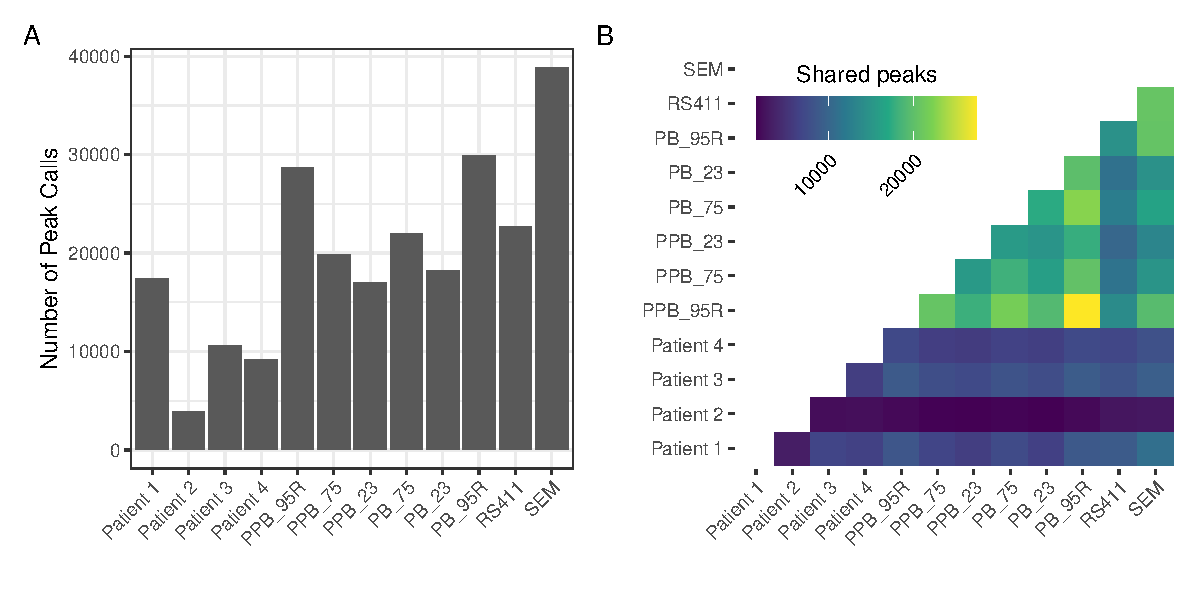
\includegraphics[width=\textwidth]{plot/ch5/mll_redo_shared_peaks.pdf}
    \caption{Peak calling of MLL-AF4 and B Cell Precursor cells with LanceOTron. A. Raw number of peak calls per cell. B. Number of shared peak calls between pairs of cells.}
    \label{fig:mll_peak_calls}
\end{figure}

% These numbers are out-dated. Not top priority to redo this. It doesn't really matter and would be similar in any case.
To justify this approach and the necessity of removing blacklisted regions, we perform the entire LDA analysis using unfiltered data, inferred topic loadings not shown. We performed region selection using the top 100, 250, and 500 regions in each topic for $k=5, \ldots, 10$ topics and found the strict overlap between the identified regions and those identified as being a part of either the ENCODE blacklist, or the ENCODE blacklist plus our custom MLL-AF4 blacklist (\Cref{fig:mll_bl_olap}). Overall, between 20.1\% and 48.8\% of the selected regions for different values of $k$ and the thresholds overlapped with ENCODE blacklisted regions. Between 51.1\% and 74.5\% of the same additionally overlapped with the custom made MLL-AF4 blacklist. 
This is compared to an overall overlap of 5998 ENCODE blacklist regions from 249903 total regions for the analysis (2.4\%) and 83434 total regions overlapping with the MLL-AF4 blacklist (33.3\%). \todo{These are from the bigwig\_merged.bed which has duplicates of the regions, so the numbers here are inflated, total is only around 63k so the others should be correspondingly less}
The blacklisted regions were therefore over-represented in the keyword regions, as expected. This analysis reaffirms the need to filter blacklisted regions.

\begin{figure}
    \centering
    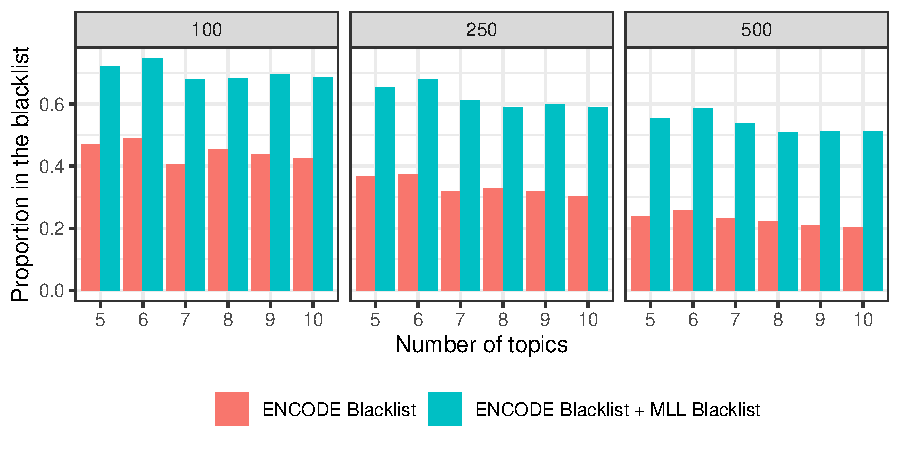
\includegraphics[width=\textwidth]{plot/ch5/mll_bl_olap.pdf}
    \caption{In an unfiltered LDA analysis of MLL-AF4 and B cell precursor cells, blacklisted regions made up the majority of identified keyword regions. Plotted is the total number of regions overlapping either of the two blacklists for a given $k$ value and the top number of regions indicated in the facet label. }
    \label{fig:mll_bl_olap}
\end{figure}

\subsubsection{Differential Accessibility between B cell Precursors and MLL-AF4 cells} \label{ch5:mll_diffacc}

After filtering out regions which overlapped with either the ENCODE or MLL-AF4 blacklist, we construct a count matrix using RPKM normalized read counts to test for baseline differential accessibility. We initially test for differential accessibility between the MLL-AF4 samples (Patients 1 through 4, RS411, and SEM) and the \gls{bcp} (PPB 1-3, PB 1-3). edgeR is used to identify differentially accessible regions between the two groups based on read counts. Overall, 27970 of the total 64162 regions were differentially accessible at a Q value threshold of 0.05. This is, however, too large a number to reasonably analyse in depth, so we select the top 100, 250, and 500 differentially accessible regions, all of which achieved statistical significance. We use GREAT to conduct an association analysis between these regions and pre-defined biological pathways. The background against which enrichment should be calculated is set to be union of all peak regions from the samples, in order to mitigate the inherent bias of analyzing accessible regions in the genome. All three subsets were enriched for Gene Ontology pathways, including peptidyl-threonine phosphorylation (4.97 fold enrichment, Q = $2.0e-7$), peptidyl-threonine modification (4.31 fold enrichment, Q = 2.4e-6), peptidyl-serine phosphorylation (2.59 fold enrichment, Q = 1.85e-2) and nucleic acid phosphodiester bond hydrolysis (2.62 fold enrichment, Q = 1.67e-2). The regions were also enriched for proximity to several genes, all of which with a corrected FDR Q value lower than 0.05 are shown in \Cref{tab:table:mll_edger_genes}.  Some of these genes are of immediate interest, including RHOU which promotes adhesion of T-cell \gls{all} cells via $\beta_1$ integrin, potentially implicating the protein in known impaired transendothelial migration potential of various kinds of leukemia cells \cite{Trinidad2009, Infante2013}. It is difficult to comprehensively survey this list of genes because their relationship with the identified regions is purely statistical. We have no mechanistic reason to believe that they are truly associated with disease. 

% Top 100, 250, and 500 motif enrichment maybe? Where are the regions?
\begin{table}

    \caption{\label{tab:table:mll_edger_genes}Enriched genic regions from the top 500 regions differentially accessible betwen MLL-AF4 cells and BCP using edgeR.}
    \centering
    \begin{tabular}[t]{llr}
    \toprule
    Gene & FDR Q Value & Fold Enrichment\\
    \midrule
    REXO1L1P & 1.41e-33 & 62.85\\ %p
    PSKH2 & 3.70e-30 & 67.37\\ 
    FOXD4L5 & 1.29e-15 & 61.60\\
    CBWD6 & 2.08e-10 & 52.50\\
    FRG2B & 4.75e-09 & 74.86\\
    \addlinespace
    RNF187 & 4.61e-09 & 51.33\\
    RHOU & 8.52e-07 & 28.52\\
    FAM27E3 & 8.54e-07 & 39.06\\
    DUX4L3 & 7.51e-06 & 128.32\\
    FOXD4L4 & 3.36e-05 & 102.66\\
    \addlinespace
    FOXD4L2 & 7.39e-05 & 29.61\\
    SERF1A & 1.94e-04 & 73.33\\
    SMN2 & 3.55e-04 & 64.16\\
    DUX4L4 & 6.23e-04 & 128.32\\
    SPATA31A5 & 2.12e-03 & 42.77\\
    \addlinespace
    ANKRD30B & 1.19e-02 & 28.52\\
    \bottomrule
    \end{tabular}
\end{table}

\subsection{Topic modelling for MLL-AF4 cells}

The focus of this chapter is an in depth investigation into using topic modelling for MLL-AF4 cells. Here, we aim to discover novel pathways that differentiate MLL-AF4 cells and normal \gls{bcp}. We do this by firstly identifying a reasonable number of topics to analyse further based on patterns in topic sharing that we observe. Secondly, we select a specific number of topics and replicate the analysis a number of times. We do this to assess the contribution of stochasticity to the inference procedure. Gibbs sampling is an approach based on Monte Carlo sampling, and as such the quality of the sampled posterior distribution can depend on the starting conditions and the convergence of the algorithm. By explicitly taking into account several repetitions of the inference algorithm we attempt to minimize the effect of chance on identified key regions. 

Similar to the above cases, peak calling is performed with LanceOTron and a score threshold of 0.5, as recommended. We construct a count matrix using the normalized read counts under each peak with BLDA as well as a one-hot encoded matrix for comparison.  Hyper-parameters alpha and beta are set for a given number of topics $k$ using Bayesian optimization and loadings are inferred using cisTopic and BLDA. 

We infer topic loadings for $k=5,\ldots,12$ topics (\Cref{fig:mll_all_topic}). The upper end of this range was chosen as the number of cells in the analysis. Increase in topic number above this point are of questionable utility, as they force more structure on the data than is present naturally.  In both the OHE and BLDA approaches, topics are identified that differentiate between the MLL-AF4 and \gls{bcp} cells. However, the topics identified by BLDA tend to be more specific, loading onto some specific cells like Patients 1 and 2, SEM/RS411, PPB, or PB predominantly. No such structure is identified in the cisTopic (right hand) case. For all values of $k$ however, at least one topic is identified for the OHE case which is predominantly active in the MLL-AF4 cells over the \gls{bcp}.

\begin{figure}
    \centering
    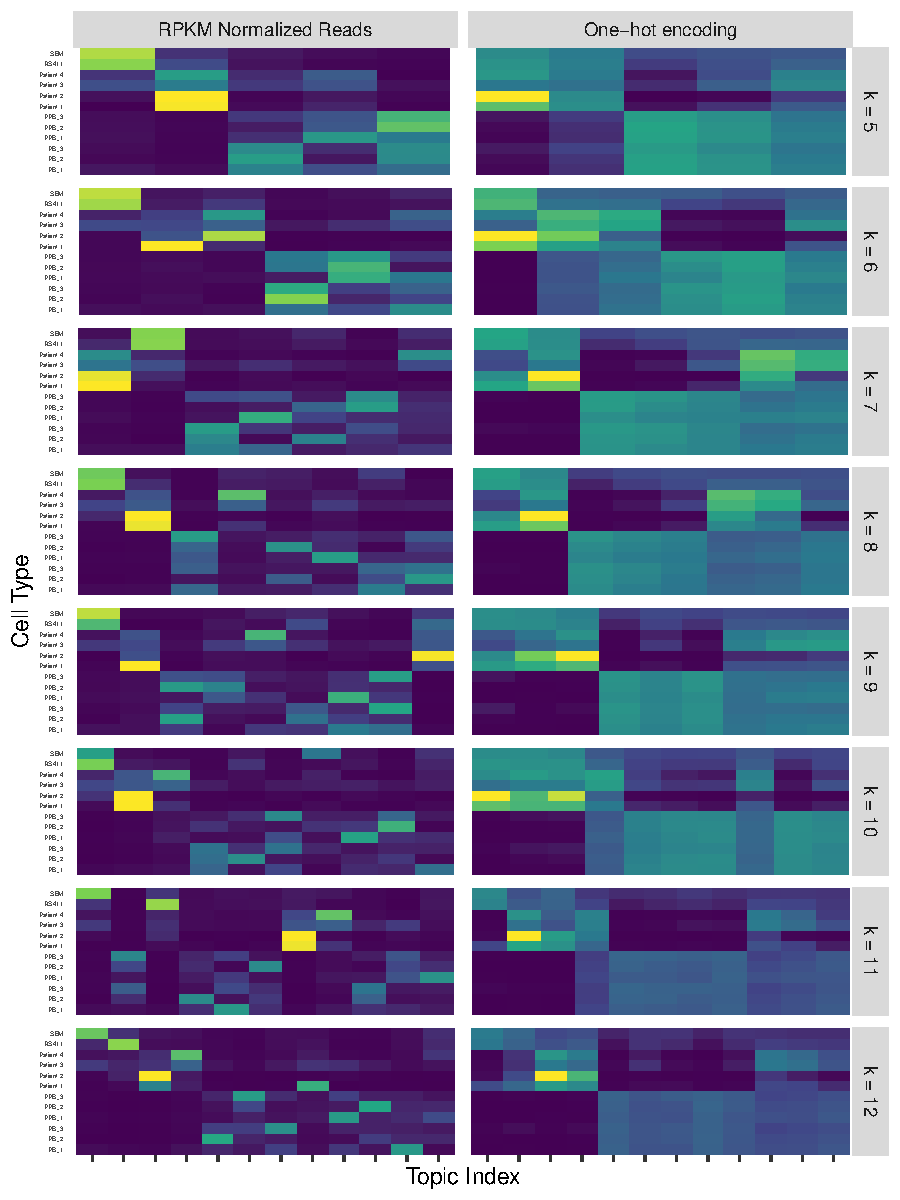
\includegraphics[width=\textwidth]{plot/ch5/mll_redo_topic_mtx.pdf}
    \caption{Inferred topic loadings for $k = 5, \ldots, 12$ topics comparing MLL-AF4 cells to B cell precursors. RPKM normalised refers to the count matrix used to infer the topic loadings by BLDA, while one-hot encoding simply annotates which regions are called as peaks by LanceOTron. Topic loadings are normalised such that the sum of all topics within a cell equals one.}
    \label{fig:mll_all_topic}
\end{figure}

Higher values of $k$ appear to impose too much structure on the data. This is evident for the BLDA case, which identifies one topic enriched for each cell type (except patient 2) at $k=12$. The OHE case interestingly deals with the over-parameterization problem differently, prefering to retain the structure seen in lower values of $k$ but assign many different topics with very low loadings within these groups. Though neither of these results are unexpected, the level of granularity for BLDA and non-specificity for OHE make it difficult to study the co-accessible regulatory elements shared between similar cell types. For that reason, we primarily are interested in the analyses for smaller values of $k$.

We select the simplest model for further analysis. We base our decision on the extremely specific topic loadings identified in the BLDA case (a single topic representing the cell lines, another involved in patients, with some sharing between them) as well as the common structure identified in PB cells separate from PPB cells with a single topic explaining the shared accessibility profile between them both. We repeat the analysis ten times for both BLDA and OHE. 

\begin{figure}
    \centering
    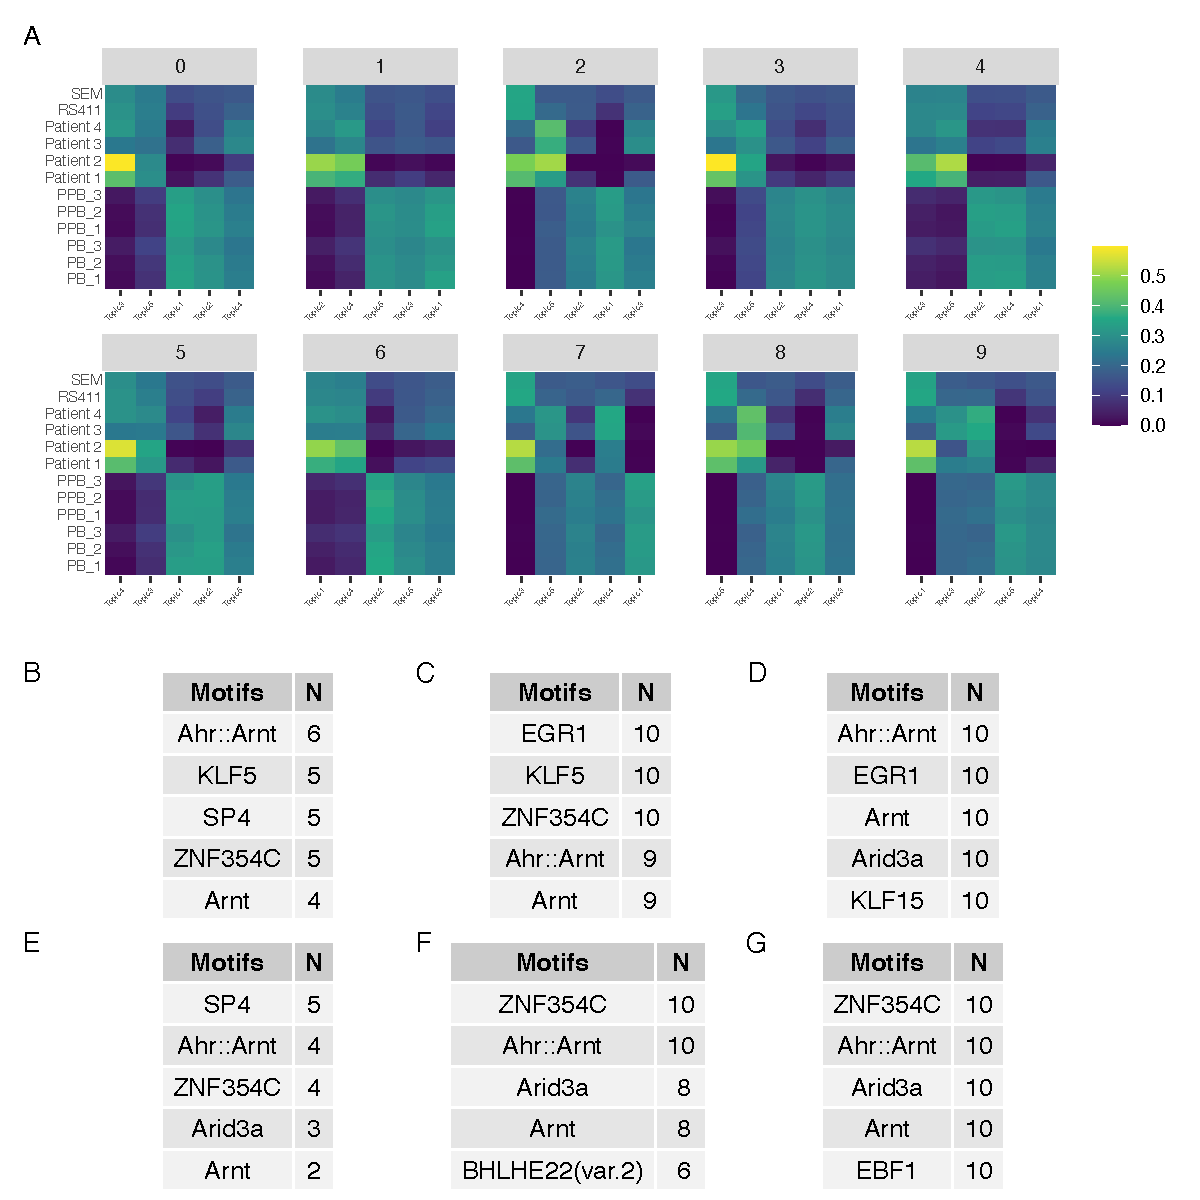
\includegraphics[width=\textwidth]{plot/ch5/mll_redo_dummy_reps.pdf}
    \caption{Ten replicates of topic modelling using one-hot encoded input. A. Inferred topic loadings on each of the samples for all 10 replicates, sorted by median topic activation. B, C, and D show the top 5 motifs identified in $N$ of the replicates in the top 100, 250, and 500 regions of manually annotated MLL-AF4 specific topics. E, F, and G show an equivalent for BCP specific topics.}
    \label{fig:mll_redo_topics}
\end{figure}

The $k=5$ OHE analysis consistently identifies at least one topic which is active in all of the MLL-AF4 cells and none of the \gls{bcp} samples (\Cref{fig:mll_redo_topics}). Patient 2 is usually the most active representative of this group within that topic. Some replicates (i.e. replicates 2, 5, 6, 7, 8, 9) also find topics active in all of the \gls{bcp} and few of the MLL-AF4 samples. There is no obvious substructure within the \gls{bcp} samples.  We manually annotate each topic as "enriched in MLL-AF4 cells", "enriched in \gls{bcp}", or neither and perform enrichment for each of the two specific sets relative to the other topics.  Motifs found in the MLL-AF4 speciifc topics in the top 100, 250, and 500 regions include SP4, KLF5, EGR1, and KLF15 (\Cref{fig:mll_redo_topics}B, C, D). Ahr::Arnt, ZNF354C, Arid3a, and Arnt are identified but found broadly between MLL-AF4 and \gls{bcp} regions.  The latter were additionally enriched for BHLHE22 and EBF1 which is a marker for B cell lineage commitment \cite{Infante2013} along with PAX5 which is occasionally identified in \gls{bcp} specific regions (data not shown). The list of motifs presented is reasonably unspecific, though there is evidence that EGR1 has deep functional relationships with many hematological malignancies including \gls{all} \cite{Tian2016}. The fact that there is at least one known system specific transcription factor whose motif is enriched for each set of samples is reassuring.  It is additionally reassuring that these important motifs were identified in each of the ten replicates in their respective sets.  Even in this low-resolution OHE setup, the technique has some power to robustly identify relevant biology across replicates.

\begin{figure}
    \centering
    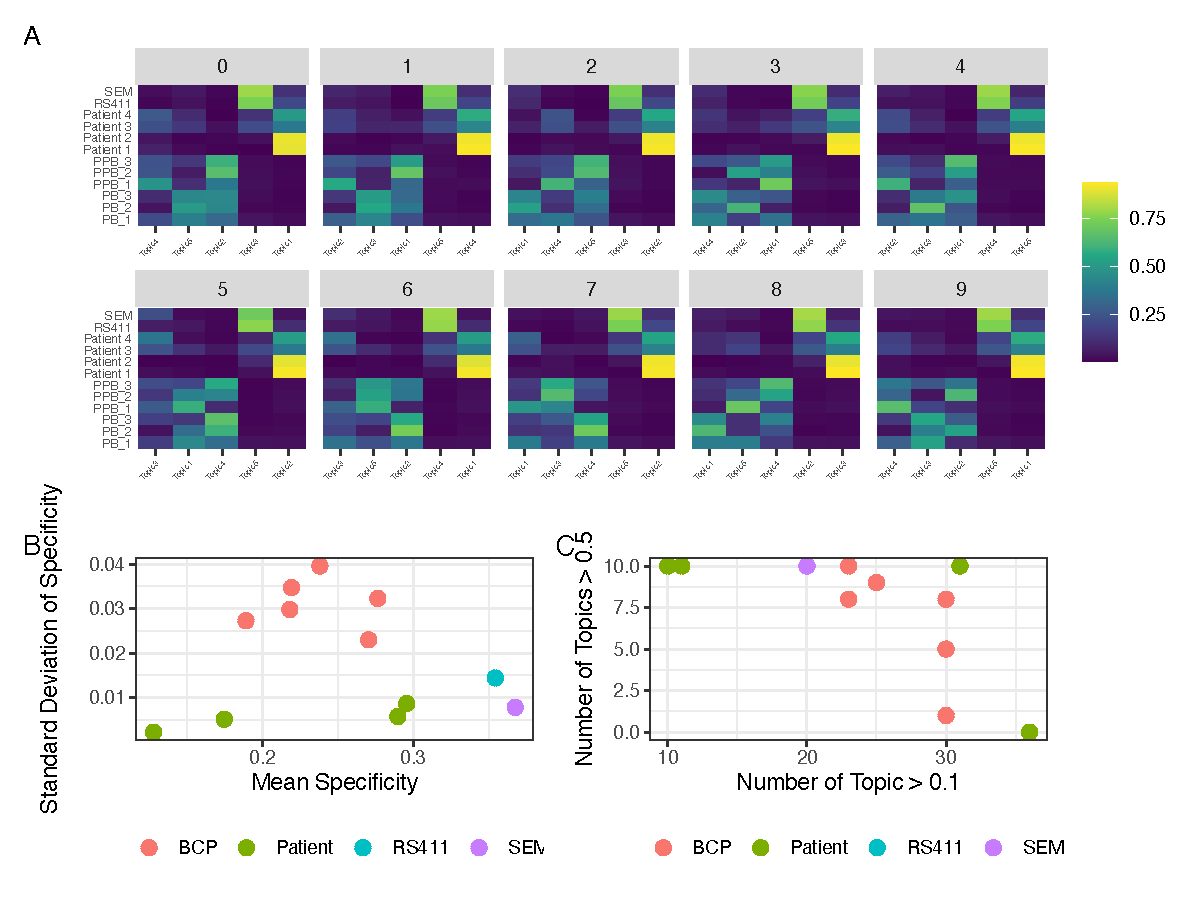
\includegraphics[width=\textwidth]{plot/ch5/mll_redo_reps_bigwig.pdf}
    \caption{Ten replicates of topic modelling using RPKM normalized input, aka BLDA. A. Inferred topic loadings for each of the 12 samples and all 10 replicates, sorted by standard deviation of topic loading. B. Mean versus standard deviation of specificity, here defined as the contribution of the most enriched topic to that sample divided by the sum of that topics enrichment to all other samples. Averaged over replicate. C. The number of instances where a sample has a topic identified above a loading value of 0.1 versus the number of instances where any topic is annotated above 0.5. Values represent contribution of a particular topic to a particular cell, such that the sum of topic loadings within a particular cell equals 1.}
    \label{fig:mll_reps}
\end{figure}

The inferred topic loadings in the BLDA case are also reproducible across replicates (\Cref{fig:mll_reps}A). In each of the 10 replicates, one topic loads preferentially onto Patients 1 and 2, and to a lesser degree onto patients 3 and 4. Another loads preferentially onto RS411 and SEM. The remainder are somewhat divided between a common co-accessibility program amongst all samples (i.e. topic 3 in replicate 5), specifically loading onto PPB (i.e. topic 5 in replicate 6), or PB (Topic 5 in replicate 0). In general, each of the replicates has at least one topic that falls into each of these categories, though the loadings onto the \gls{bcp} are less consistent than the MLL-AF4 cells. The topics loading onto RS411 and SEM were highly specific to those two samples, in contrast to the BCPs whose specificity was much lower, and additionally much more variable (\Cref{fig:mll_reps}B).  The BCPs additionally had many topics annotated to them at low levels, but very few with a higher annotation level of 0.5 (\Cref{fig:mll_reps}C).  This is in contrast to Patients 1 and 2, who had both a large number of highly specific topics across the replicates, and also a very low number of non-specific topics.  From this we conclude that similar topics are able to be found consistently across replicates.  

Having established a high degree of specificity for individual topics to the expected annotations of the samples, we investigate the regions making up the topics. We briefly focus on a single replicate, indexed as 0 in \Cref{fig:mll_reps}. An interesting avenue for exploration is the degree to which the topics are made up of similar regions. If they were, it would represent a shared core of co-accessible elements. The alternative, of completely separate underlying regions, is equally interesting. An understanding of the region-topic distribution over cell types will aid in the interpretation of the key regions for particular topics. We transform each region-topic vector to $Z$-scores by subtracting the mean and dividing by the standard deviation of the distribution, and count the number of regions with a $Z$-score over 3 (98.8 percentile of a theoretical standard normal distribution) in each of the topics (diagonal of \Cref{fig:mll_region_sharing}A). We additionally count the regions with a $Z$ score of 3 or higher in both of two different topics and find generally low region sharing overall, except in the case of topics 2 and 5 where 330 regions were enriched for both(off-diagonal elements of \Cref{fig:mll_region_sharing}A). Topics 2 and 5 in this replicate were enriched for PB cells and all BCP respectively. The regions selected as a part of this set had higher read counts in BCP samples than MLL-AF4 samples (\Cref{fig:mll_region_sharing}B).  This indicates a high degree of co-accessibility between important regions in PB and PPB cells. In contrast to this, few regions were shared between the two MLL-AF4 topics. The regions with topic 1 loadings over a $Z$ score of three were more accessible in the patient samples, though this was not a statistically significant difference (\Cref{fig:mll_region_sharing}C). However, the small number of important regions for the RS411/SEM topic were more accessible in these cell types (\Cref{fig:mll_region_sharing}).

\begin{figure}
    \centering
    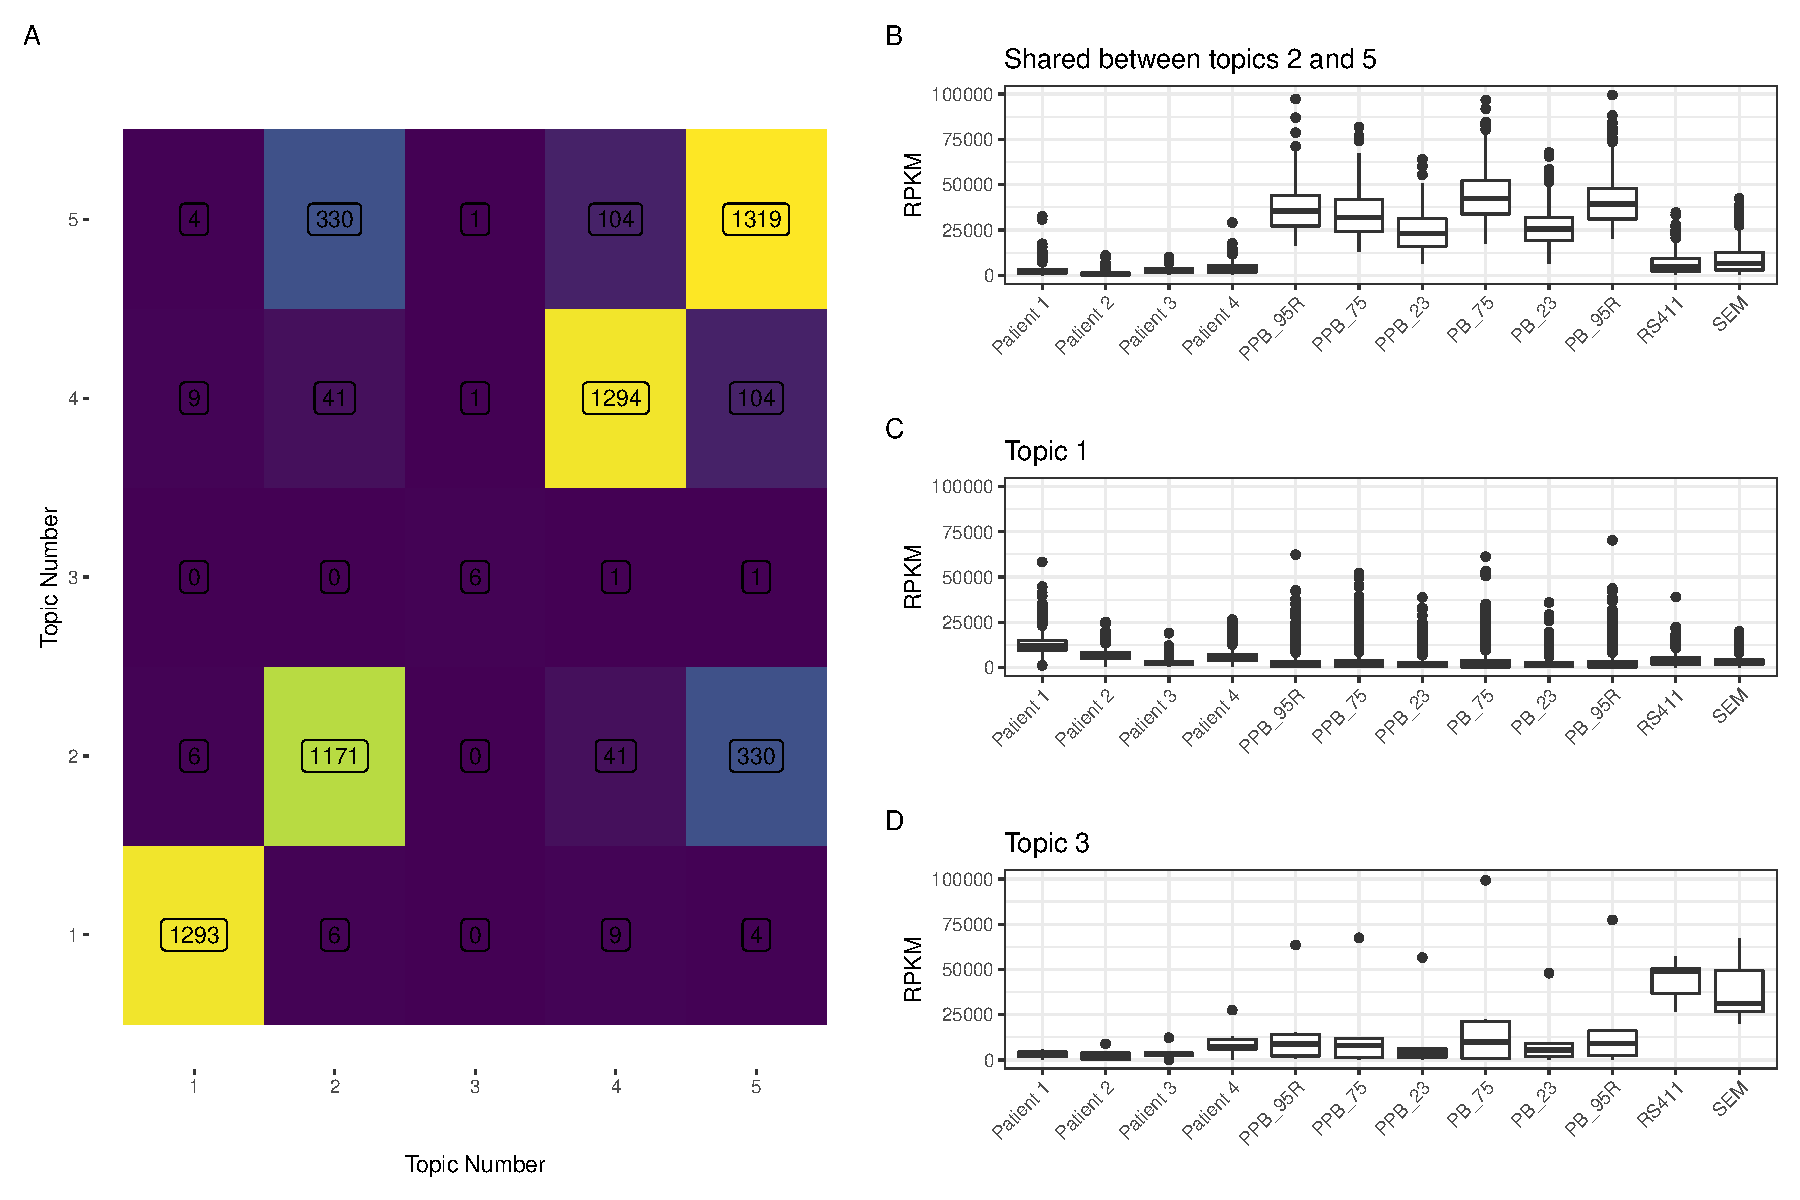
\includegraphics[width=\textwidth]{plot/ch5/mll_bigwig_region_sharing_plot_rep0.pdf}
    \caption{Regions highly annotated on each of the five topics in replicate 0 for the BLDA topic modelling. A. Region-topic loadings were converted to Z scores by subtracting the mean of the distribution and dividing by the standard deviation. Regions with a $Z$ score of 3 or more were selected, and the number of shared highly loaded regions is plotted. The number identified per topic is plotted on the diagonal. B. RPKM values for the 330 regions highly loaded for both topics 2 and 5. In this replicate, these topics were enriched in BCPs. C. RPKM values for regions highly loaded with topic 1, which primarily loads onto patient samples. D. RPKM values for the 6 regions highly loaded with topic 3, which is enriched in RS411 and SEM samples.}
    \label{fig:mll_region_sharing}
\end{figure}


We sought to understand how reproducibly these regions were identified between replicates. 
Regions robustly identified as being associated with a topic that loads highly onto a desirable set of samples represent key candidates for further investigation.
We identified the top 100, 250, and 500 regions for each topic in each replicate, and found how many of these regions are shared between 8, 9, or all of the replicates (\Cref{fig:mll_region_repro}A). Patients have the highest key-word topic reproducibility across replicates, with 76 of the top 100 identified in every single replicate. The patient group has the lower number of unique regulatory elements identified for any threshold (\Cref{fig:mll_region_repro}B). Amongst the 76 reproducibly identified regions, average expression is almost threefold higher in patients than the remainder of samples (mean of patients = 11321.8, mean of other = 4291.5, Student's $T$-test $P$ value for difference < 2.2e-16). These regions therefore represent a prioritized set that is both important for the highly-specific topic modelling approach and identified in each of the ten replicates. 

Deriving some idea of functional characteristics from an abitrary set of genomic regions is difficult. Evolutionary conservation, biochemical properties such as histone modifications, and studying genetic mutations can all lend some degree of credibility linking a collection of regions to a particular pathway of interest \cite{Kellis2014}. Within the context of this sample, understanding the role of these regions is additionally confounded by the fact that they are derived from blastic, malignant cancer cells. Practically, this means that they may contain somatic mutations not represented in the reference panel. At present, there is no reliable, published, method for calling mutations from peak-based NGS experiments. Even if this data were available, it would be difficult to differentiate between accessibility as a consequence of cellular environment and differential evolution from that caused by genetic differences. The interpretation of the functional role of regions identified herein is hampered by a lack of functional validation due to the timelines imposed on this thesis.  

\begin{figure}
    \centering
    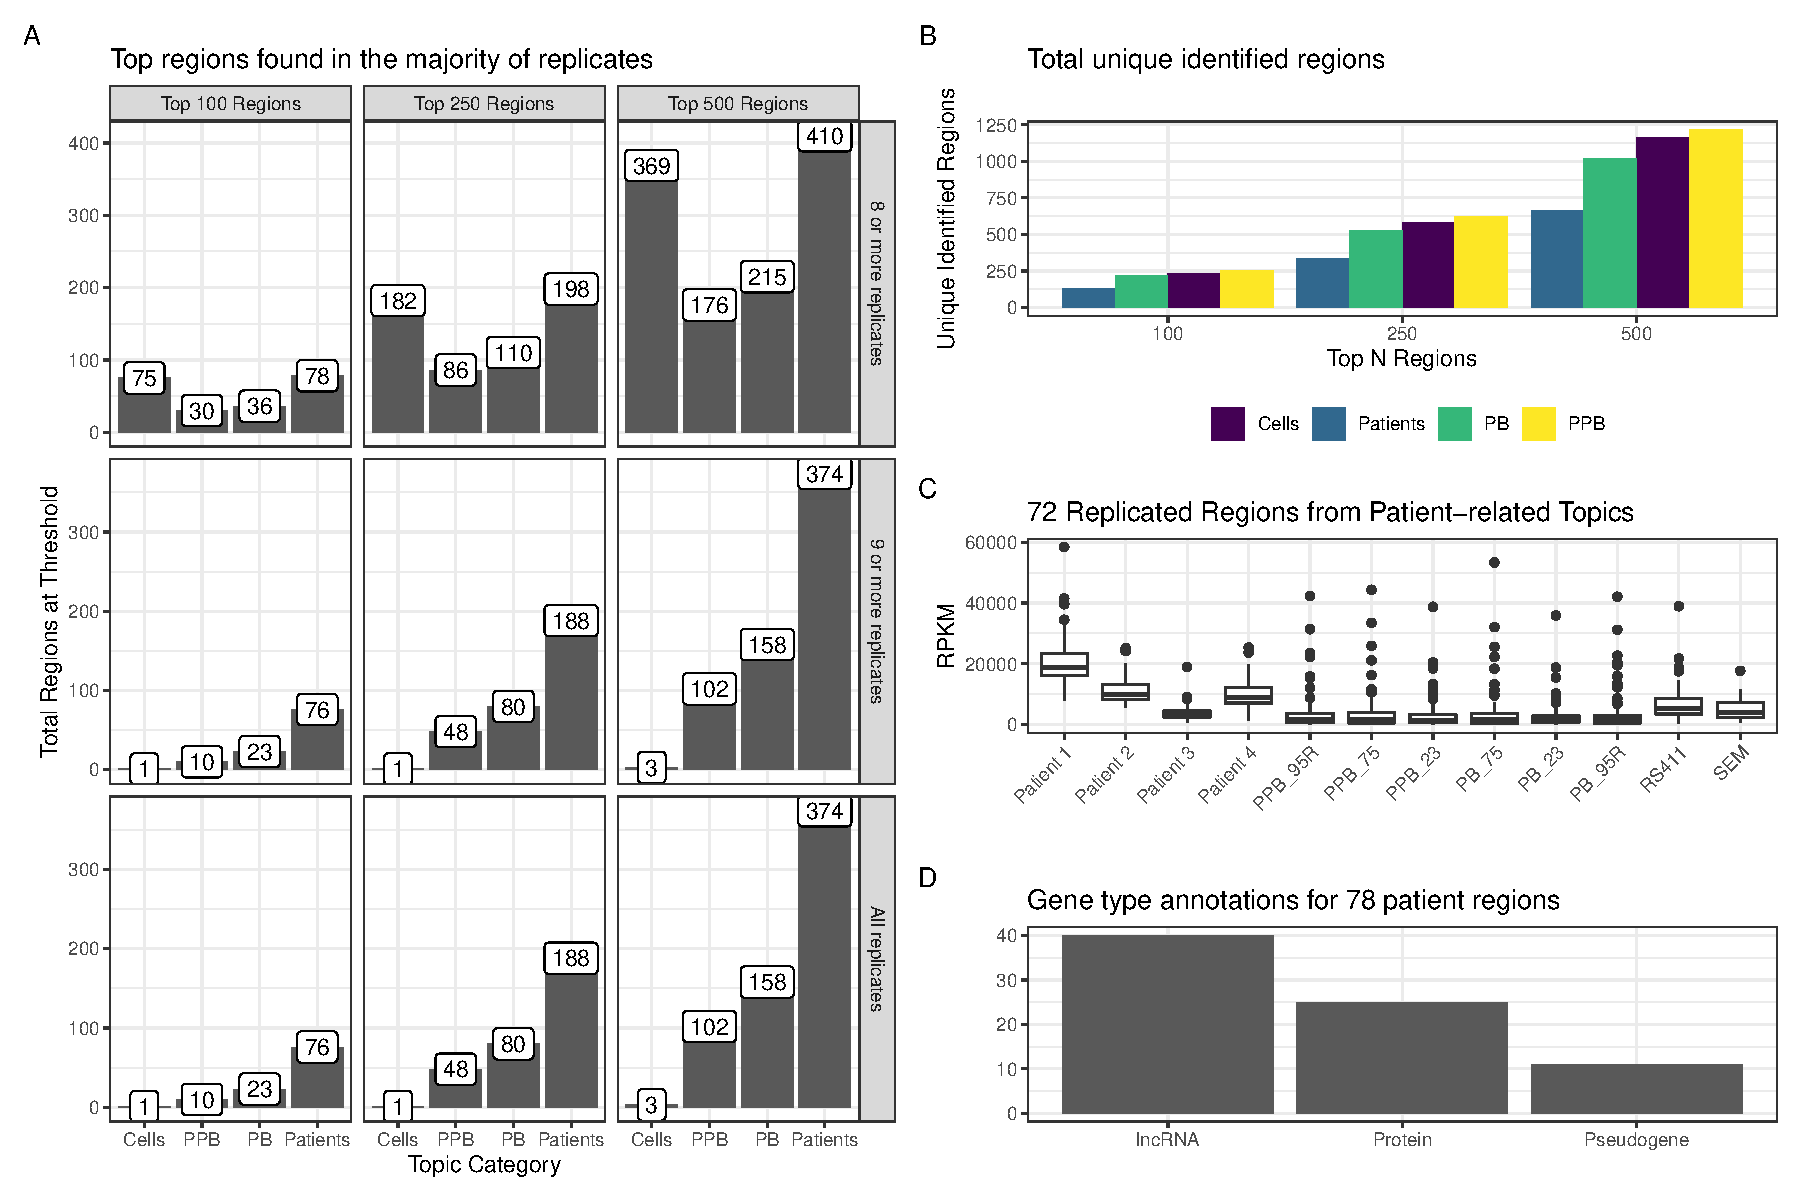
\includegraphics[width=\textwidth]{plot/ch5/mll_top_regions_bigwig.pdf}
    \caption[A subset of patient specific regions are highly reproducible across replicates and are enriched for lncRNA genes.]{A subset of patient specific regions are highly reproducible across replicates and are enriched for lncRNA genes. A. For each of the 100, 250, or 500 top regions per manually annotated sample specific topic, the number of regions occuring in eight or more, nine or more, or all of the ten replicates is plotted. B. The intersection of all regions identified across replicates for each set of sample-specific topics. C. RPKM profile for the 76 regions identified in A as being highly reproducible. D. Gene type annotation from refseq for closest annotated genes for the same regions.}
    \label{fig:mll_region_repro}
\end{figure}

We begin our characterization of these regions by finding their closest annotated gene body. 32 of the 76 regions lie directly within genic regions. The remainder tend to be found within 50kb of the nearest gene, but the distance is highly variable and some regions are as far as 200kb from their closest gene (\Cref{fig:mll_lnc}A). This distance distribution fits well to our expectations if the regions represented inter-genic enhancer elements.  The closest annotated genes are, interestingly, \glspl{lnc}, and are found in a much higher frequency than expected in 76 randomly samples genes (\Cref{fig:mll_lnc}B,C). Though this result is suggestive, \glspl{lnc} are very challenging to correctly annotate, with efforts being confounded by both technical artifacts and methodological complications \cite[see Figure 1 for an overview of challenges associated with lncRNA annotation]{Cao2018}. There is, however, growing evidence that cancer cells, including leukemic blasts, may hijack the large and poorly understood lncRNA transcriptome to influence differentiation, energy metabolism, malignant proliferation, apoptosis, and the drug resistance of leukemia cells \cite[Table 1]{Gao2020}. It is possible, therefore, that the regions identified represent \glspl{cre} influencing the expression of functional lncRNAs involved in each individual patient's leukemia. However, none of the lncRNAs identified match with those in Table 1 of \textcite{Gao20202}, so their potential functions will remain the subject of further investigation.

\begin{figure}
    \centering
    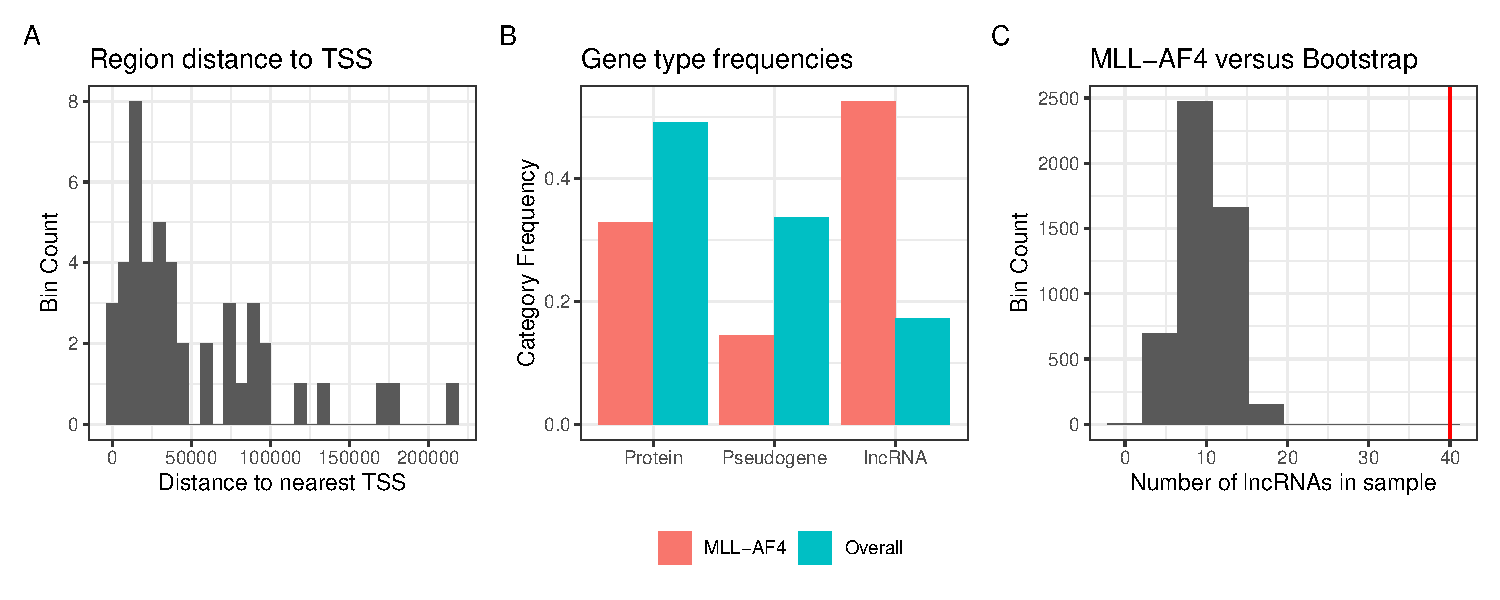
\includegraphics[width=\textwidth]{plot/ch5/mll_lnc.pdf}
    \caption{MLL-AF4 regions compared to reference genes. A. Distance of the 76 reproducible patient regions to their nearest annotate TSS, minus the regions which are sitting in genic regions. B. Frequencies of gene categories in refSeq versus the sample of closest patient genes. C. Frequency of lncRNAs in 5000 random samples of 76 regions from refSeq, showing that the observed frequency of lncRNA is in the far tail of this distribution.}
    \label{fig:mll_lnc}
\end{figure}

Histone proteins within nucleosomes may be post-translationally modified by the addition of several chemical groups which collectively serve to regulate transcription and the recruitment of transcription factors. The presence of specific histone modifications at a particular location of the genome can be determined experimentally using \gls{chip}, where peak regions give an estimate of the presence or absence of a particular modification. There are many histone modifications, and their combinatorial method of action makes it difficult to interpret the exact ramifications of their presence \cite{T2001}. Previously, a small number of important histone modifications and transcription factor binding sites were characterized in these samples (see Methods).  

We called peaks on each of the ChIP-seq tracks using LanceOTron and intersected the peaks with the reproducible set of patient regions. We additionally drew 1000 random samples from the set of accessible regions used in this section, creating an empirical P-value, to understand the relative enrichment of these ChIP-seq signals versus the genomic background of accessible sequence. Within the available ChIP-seq data, regions are relatively enriched for H3K27ac, H3K4me1, and H3K4me3 (\Cref{table:mll_chip}). They are depleted in K379me2, and there is evidence that we see more binding of MLL to these regions than we would expect by chance, especially in patient 11911, where we additionally see increased binding of AF4, PAF1c, and RUNX1. The relative abundance of H3K27ac and H3k4me1 indicate that these elements may be acting as enhancers. However, it is not clear whether the high abundance of PAF1c, RUNX1, and MLL marks are due to general enrichment in enhancer regions or are somehow associated with these regions functionally. As patient 11911 is the only available sample with all of these chromatin marks and transcription factors available, we elect to study this patient specifically. We create a set of putative enhancer elements by selecting 18101 regions from the total 64162 accessible regions that overlap with both H3K27ac and H3K4me1 peaks. We then perform a similar analysis to before, selecting 5000 sets of 76 regions at random and observing the proportion of the putative enhancer elements that are additionally bound by MLL, AF4, PAF1c, and RUNX1. The resulting distributions show that none of the 5000 random samples are as highly enriched for MLL, PAF1c, or RUNX1 as the reproducible patient regions (\Cref{fig:mll_enhancer_overlap}). MLL binding is enriched by approximately 50\% over the mean of the distribution (67 versus 44.8), RUNX1 binding is 63\% higher than the mean (48 versus 29.3), and PAF1c is enriched by nearly 70\% (52 versus 30.6). We discuss the relevance of these transcription factors in the Discussion section. 

\begin{figure}
    \centering
    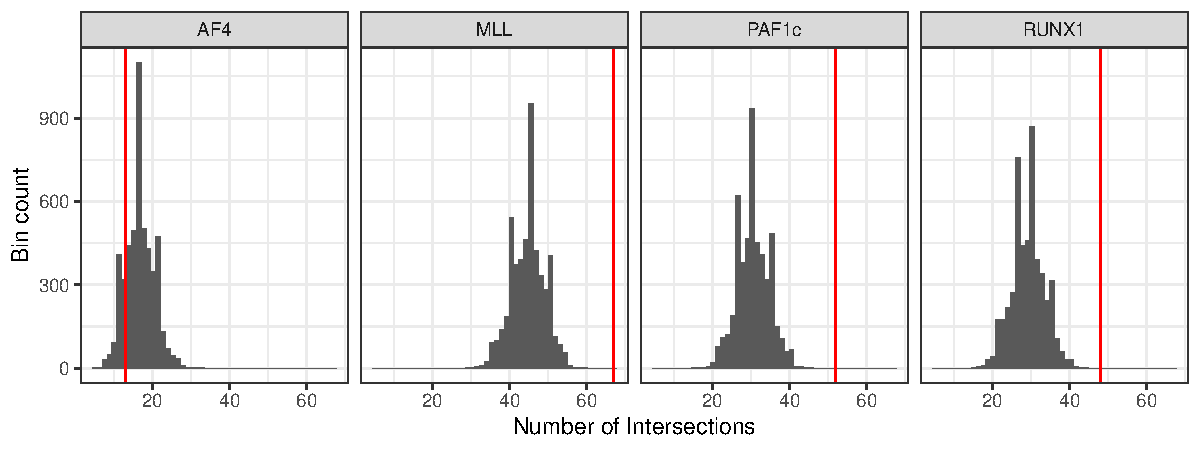
\includegraphics[width=\textwidth]{plot/ch5/mll_enhancer_overlap.pdf}
    \caption{Number of intersections between 76 randomly selected putative enhancer sites (accessible regions which overlapped with both H3K4me1 and H3K27ac chromatin peaks) in 5000 random samples compared to the observed quantities in the reproducible patient regions (plotted in red as a vertical line).}
    \label{fig:mll_enhancer_overlap}
\end{figure}

\begin{figure}
    \centering
    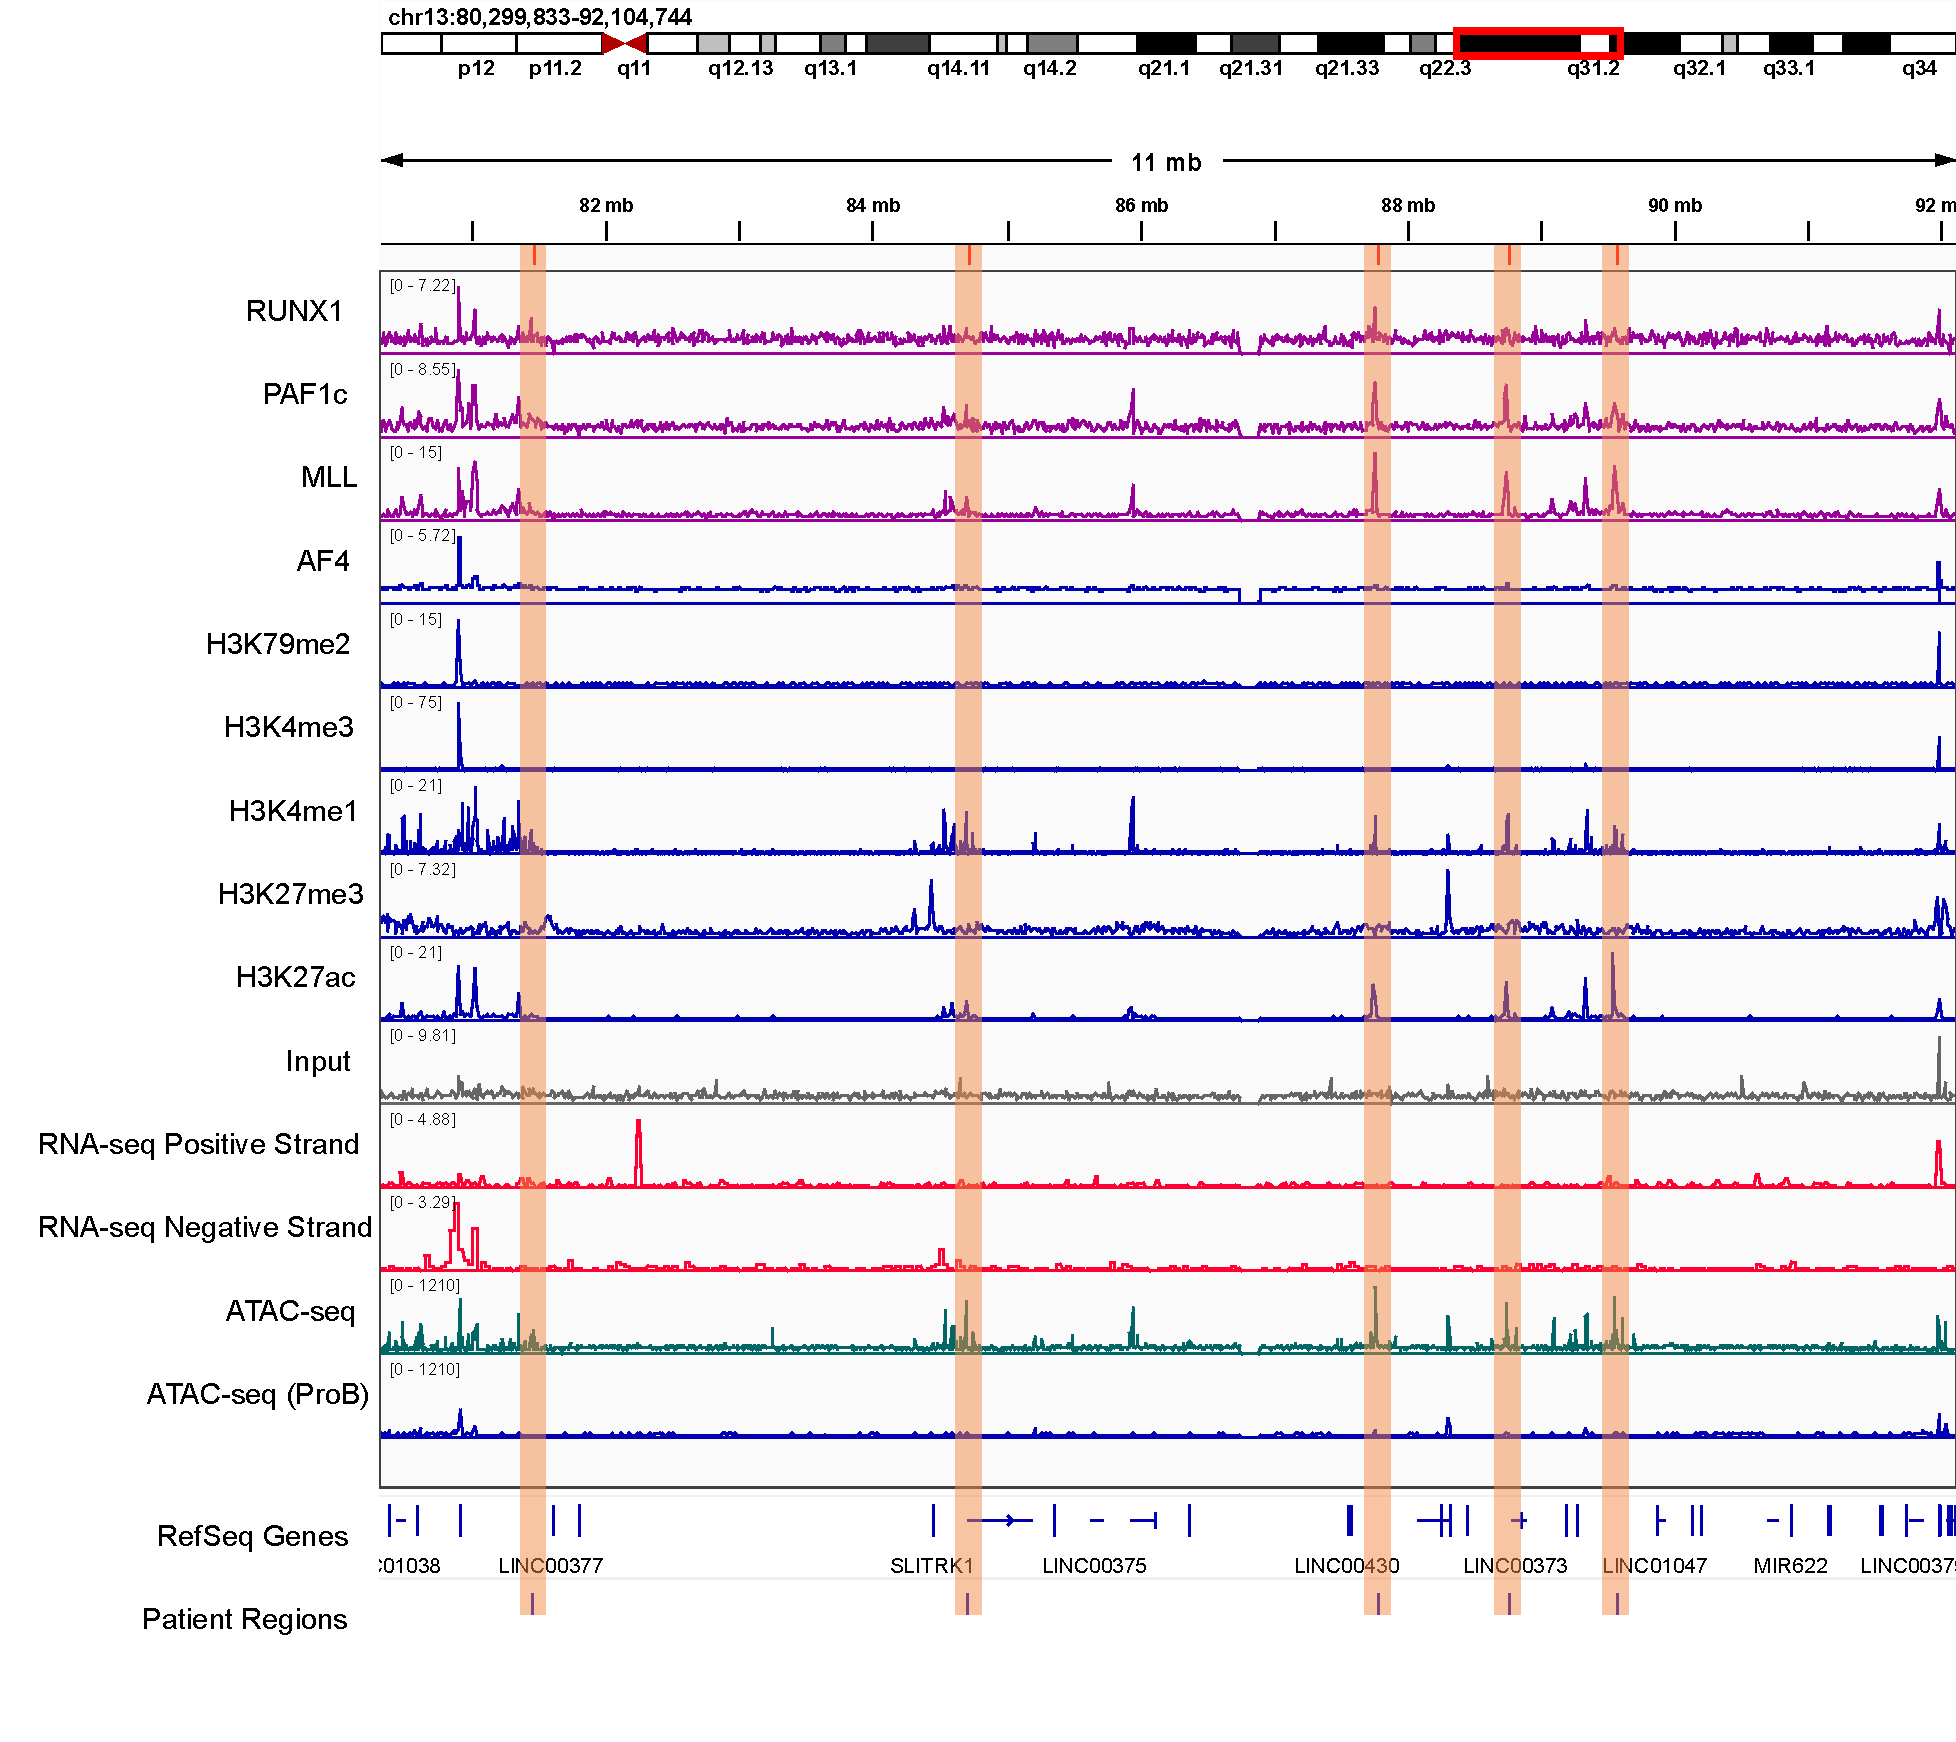
\includegraphics[width=\textwidth]{plot/ch5/enhancer_cluster.pdf}
    \caption{Coverage tracks for ChIP-seq marks, RNA-seq, and ATAC-seq for patient 11911 as well as PB cell for comparison. Five regions are in close promiximity to each other, each marked with H3K4me1, H3K27ac, MLL, and PAF1c. Regions of interest are highlighted in orange, with the highlight extending slightly beyond their borders for visual clarity.}
    \label{fig:mll_enhancer_cluster}
\end{figure}


\begin{table}

    \centering
    \tiny
    \begin{tabular}[t]{llllllllll}
    \toprule
    Patient ID & H3K27ac & H3K4me1 & H3K4me3 & H3K79me2 & MLL & AF4 & H3K27me3 & PAF1c & RUNX1\\
    \midrule
    26754 & 57 (0) & 60 (0) & 31 (0) & 2 (0.968) & 42 (0) & 4 (0.631) &   &   &  \\
    11911 & 66 (0) & 72 (0) & 32 (0) & 2 (0.975) & 67 (0) & 13 (0.004) & 1 (0.933) & 52 (0) & 48 (0)\\
    27800 & 60 (0) & 61 (0) & 38 (0) & 3 (0.956) &   &   &   &   &  \\
    25911 & 23 (0) &   &   &   & 24 (0) &   &   &   &  \\
    \bottomrule
    \end{tabular}
    \caption{ChIP-seq peak overlaps with reproducible patient regions, with the proportion of overlaps from 1000 random draws from all accessible regions in brackets. }
    \label{table:mll_chip}
    \end{table}


\begin{table}[]
    \tiny
    \begin{tabularx}{\textwidth}{lllX}
    \toprule
    Region                                     & Function                   & Gene        & Cell line reference                                                             \\ \midrule
    chr1:239881927-239883919                   & Promoter                   & CHRM3-AS2   &                                                                                 \\
    \multirow{4}{*}{chr2:133023823-133025309}  & \multirow{4}{*}{Enhancer}  & AC098826.5; & GM19238;                                                                        \\
                                               &                            & CDC27P1;    & GM19238,Pancreatic\_islet;                                                      \\
                                               &                            & GPR39;      & Pancreatic\_islet;                                                              \\
                                               &                            & LYPD1       & Pancreatic\_islet                                                               \\
    \multirow{4}{*}{chr3:97628722-97630587}    & \multirow{4}{*}{Enhancer}  & ARL6;       & HT29;                                                                           \\
                                               &                            & AC110491.1; & HT29;                                                                           \\
                                               &                            & CRYBG3;     & HT29,PC3,th1,Thymus;                                                            \\
                                               &                            & MINA        & HT29,Mesendoderm,NB4,PC3                                                        \\
    \multirow{9}{*}{chr3:160554953-160556142}  & \multirow{9}{*}{Enhancer}  & IFT80;      & HT29;                                                                           \\
                                               &                            & RP11;       & HT29,NB4;                                                                       \\
                                               &                            & TRIM59;     & HT29;                                                                           \\
                                               &                            & SCARNA7;    & HT29;                                                                           \\
                                               &                            & ARL14;      & HT29;                                                                           \\
                                               &                            & RP11;       & HT29,NB4;                                                                       \\
                                               &                            & PPM1L;      & HT29,NB4;                                                                       \\
                                               &                            & RP11;       & HT29,NB4;                                                                       \\
                                               &                            & NMD3        & NB4                                                                             \\
    \multirow{10}{*}{chr3:190303470-190305623} & \multirow{10}{*}{Enhancer} & IL1RAP;     & HFF,hMADS-3,HT29,Keratinocyte,MCF10A,\newline melanoma,Mesendoderm,NB4,PC3,T98G,ZR75-30; \\
                                               &                            & GCNT1P3;    & hMADS-3,Keratinocyte,MCF10A,melanoma,NB4;                                       \\
                                               &                            & 7SK;        & hMADS-3,Keratinocyte,MCF10A,melanoma,NB4;                                       \\
                                               &                            & MTAPP2;     & HT29,Keratinocyte,Mesendoderm,T98G;                                             \\
                                               &                            & CLDN1;      & HT29,Keratinocyte,MCF10A,PC3;                                                   \\
                                               &                            & LEPREL1;    & Keratinocyte,MCF10A,Mesendoderm;                                                \\
                                               &                            & CLDN16;     & Keratinocyte,NB4;                                                               \\
                                               &                            & CCT6P4;     & Keratinocyte,NB4;                                                               \\
                                               &                            & TMEM207;    & NB4;                                                                            \\
                                               &                            & RP11        & NB4                                                                             \\
    \multirow{8}{*}{chr4:54721244-54722456}    & \multirow{8}{*}{Enhancer}  & RP11;       & HFF,ZR75-30;                                                                    \\
                                               &                            & LNX1;       & HFF;                                                                            \\
                                               &                            & RP11;       & HFF,ZR75-30;                                                                    \\
                                               &                            & CHIC2;      & HFF,ZR75-30;                                                                    \\
                                               &                            & RP11;       & HFF,ZR75-30;                                                                    \\
                                               &                            & PDGFRA;     & HFF;                                                                            \\
                                               &                            & RPL21P44;   & ZR75-30;                                                                        \\
                                               &                            & MORF4L2P1   & ZR75-30                                                                         \\
    \multirow{3}{*}{chr4:177823634-177824977}  & \multirow{3}{*}{Enhancer}  & SPCS3;      & HFF;                                                                            \\
                                               &                            & RP11;       & HFF,LHCN-M2,SK-N-SH\_RA;                                                        \\
                                               &                            & NEIL3       & Keratinocyte,MCF10A                                                             \\
    chr5:82663769-82665217                     & Enhancer                   & TMEM167A    & ZR75-30                                                                         \\
    \multirow{3}{*}{chr5:119723091-119724865}  & \multirow{3}{*}{Enhancer}  & PRR16;      & HFF;                                                                            \\
                                               &                            & CTD;        & HFF,LHCN-M2;                                                                    \\
                                               &                            & RP11        & melanoma                                                                        \\
    \multirow{2}{*}{chr6:141130170-141131796}  & \multirow{2}{*}{Enhancer}  & RP3;        & ME-1;                                                                           \\
                                               &                            & RP11        & ME-1                                                                            \\
    chr6:161161634-161163661                   & Enhancer                   & PLG         & GM12891,Namalwa                                                                 \\
    chr7:11870320-11872428                     & Promoter                   & THSD7A      &                                                                                 \\
    chr7:81474664-81476523                     & Enhancer                   & MIR1255B1   & NB4                                                                             \\
    \multirow{3}{*}{chr8:77492793-77494807}    & \multirow{3}{*}{Enhancer}  & MRPL9P1;    & ESC\_neuron,SK-N-SH\_RA;                                                        \\
                                               &                            & ZFHX4;      & ESC\_neuron;                                                                    \\
                                               &                            & RP11        & ESC\_neuron,SK-N-SH\_RA                                                         \\
    chr9:42018481-42020192                     & Promoter                   & \multicolumn{2}{l}{LOC102724238,LOC554249,KGFLP2}                                             \\
    chr9:46686996-46688539                     & Promoter                   & \multicolumn{2}{l}{KGFLP1,LOC554249,LOC102724238}                                             \\
    \multirow{8}{*}{chr10:33654161-33655412}   & \multirow{8}{*}{Enhancer}  & AK3P5;      & FT246,HFF,hMADS-3,HT29,LHCN-M2,ZR75-30;                                         \\
                                               &                            & RP11;       & FT246,FT33,HFF,hMADS-3,HT29,Keratinocyte,LHCN-M2,ZR75-30;                       \\
                                               &                            & RP11;       & FT246,FT33,HFF,hMADS-3,HT29,Keratinocyte,LHCN-M2,ZR75-30;                       \\
                                               &                            & ITGB1;      & FT246,FT33,HFF,hMADS-3,HT29,Keratinocyte,LHCN-M2,ZR75-30;                       \\
                                               &                            & RP11;       & FT246,FT33,HFF,hMADS-3,HT29,Keratinocyte,LHCN-M2,ZR75-30;                       \\
                                               &                            & RP11;       & FT246,FT33,HFF,hMADS-3,HT29,Keratinocyte,LHCN-M2,ZR75-30;                       \\
                                               &                            & NRP1;       & FT246,FT33,HFF,hMADS-3,LHCN-M2;                                                 \\
                                               &                            & AL353600.1  & hMADS-3                                                                         \\
    chr10:58119756-58122125                    & Promoter                   & ZWINT       &                                                                                 \\
    chr12:24531253-24532422                    & Enhancer                   & BCAT1       & hMADS-3,Mesendoderm                                                             \\
    \multirow{2}{*}{chr13:54602807-54604709}   & \multirow{2}{*}{Enhancer}  & LINC00458;  & Mesendoderm;                                                                    \\
                                               &                            & RPL13AP25   & Mesendoderm                                                                     \\
    chr13:84710151-84712348                    & Promoter                   & LINC00333   &                                                                                 \\
    \multirow{5}{*}{chr13:103658908-103660657} & \multirow{5}{*}{Enhancer}  & TPP2;       & GM19238,GM19239,HFF,Namalwa;                                                    \\
                                               &                            & KDELC1;     & GM19238,GM19239,HFF,Namalwa;                                                    \\
                                               &                            & BIVM;       & GM19238,GM19239,HFF,Namalwa;                                                    \\
                                               &                            & ERCC5;      & GM19238,GM19239,HFF,Namalwa;                                                    \\
                                               &                            & TEX30       & HFF,Namalwa                                                                     \\
    \multirow{2}{*}{chr14:38593423-38595439}   & \multirow{2}{*}{Enhancer}  & CTD;        & Mesendoderm;                                                                    \\
                                               &                            & SSTR1       & Mesendoderm                                                                     \\ \cmidrule(l){1-4} 
    \end{tabularx}
    \caption{EnhancerAtlas 2.0 results for the 76 reproducibly identified patient regions.}
    \label{table:mll_enhancer}
    \end{table}



% discuss this in the discussion, don't interperet it here.
We searched EnhancerAtlas 2.0 (Citation) for regions matching ours, and found that 17 out of the 76 regions were known enhancers, and 6 were known promoters (\Cref{table:mll_enhancer}). The functionality validated active cell types varied considerably, from enhancers for GPR39 and LYPD1 in pancreatic islet cells to more similar TMEM207 and RP11 enhancers in pro-myelotic leukemia cell line NB4. In this list as well, non-coding RNA targets are also over-represented. RP11, for example, was identified as functionally validated target of 10 of the 17 enhancers. Though RP11 represents a class of otherwise unannotated genes, rather than a protein of its own, many subtypes of RP11 are in fact non-coding RNAs (CITATION). As previously mentioned, these regions are clearly marked as putative enhancer regions, though it is not immediately obvious which genes they may be regulating. Interestingly, some regions co-occur in clusters such as the one on Chromosome 13 in \Cref{fig:mll_enhancer_cluster}. Here, five regions are found together, each marked with enhancer marks H3K4me1 and H3K27ac as well as the transcription factors MLL and PAF1c. The second of these five regions is annotated as an enhancer for TPP2, KDELC1, BIVM, ERCC5, and TEX30 in GM EBV-immortalized cells as well as a fibroblast cell line HFF-1. Whether the remainder of the enhancers are novel in the MLL-AF4 patients remains to be shown experimentally, however there is no clear accessibility in these regions for \glspl{bcp}. Interestingly, these regions are all most accessible in patients compared to any other cell type in the ENCODE blood cell type collection, suggesting that their function may be new in these patient samples (\Cref{fig:encode_pt_regions}). 

\begin{figure}
    \centering
    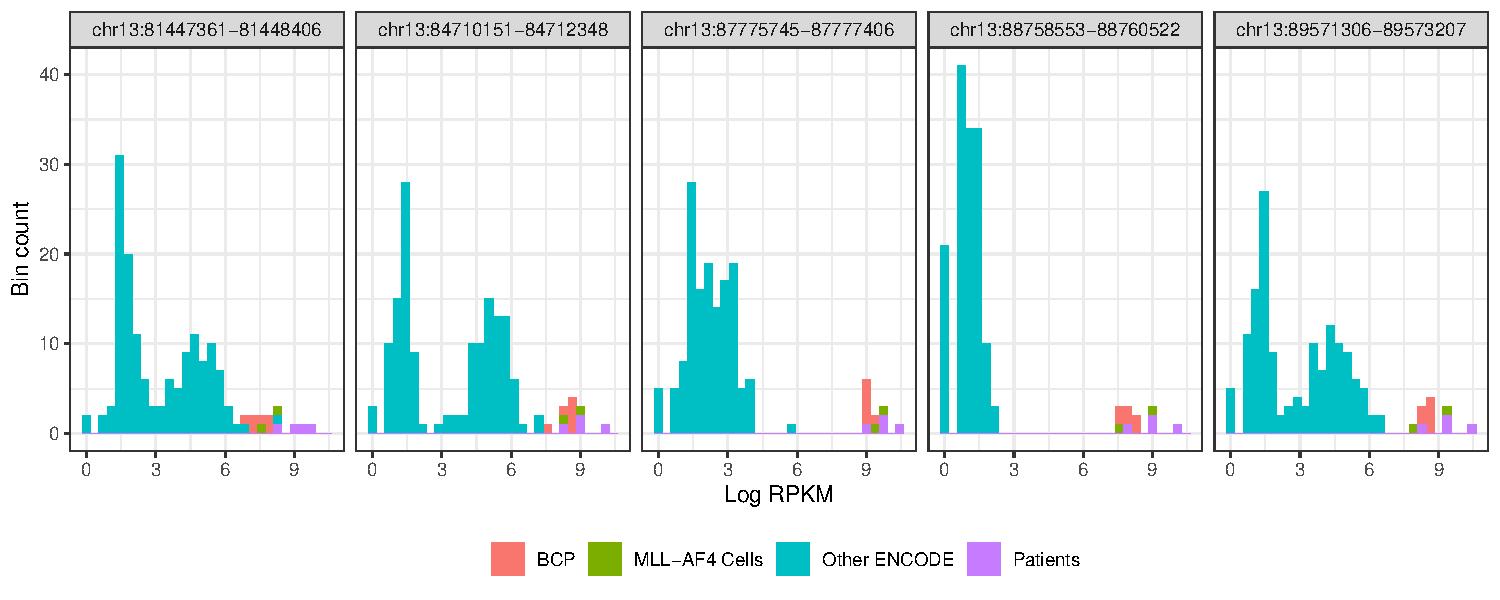
\includegraphics[width=\textwidth]{plot/ch5/pt_compared_to_encode.pdf}
    \caption{Log RPKM for five regions in a putative enhancer cluster identified through topic modelling in ENCODE blood cells versus patients and MLL-AF4 cell types.}
    \label{fig:encode_pt_regions}
\end{figure}


% For tomorrow

- 55 of the regions from the patient topic are also found in the encode when you take out anything active in other cell types.
- are these also the ones actually marked by things and therefore active? 

- Correspondance between the RS411 and SEM topics just in a summary way
- Use the ENCODE as basically a replication

%\begin{figure}
%    \centering
%    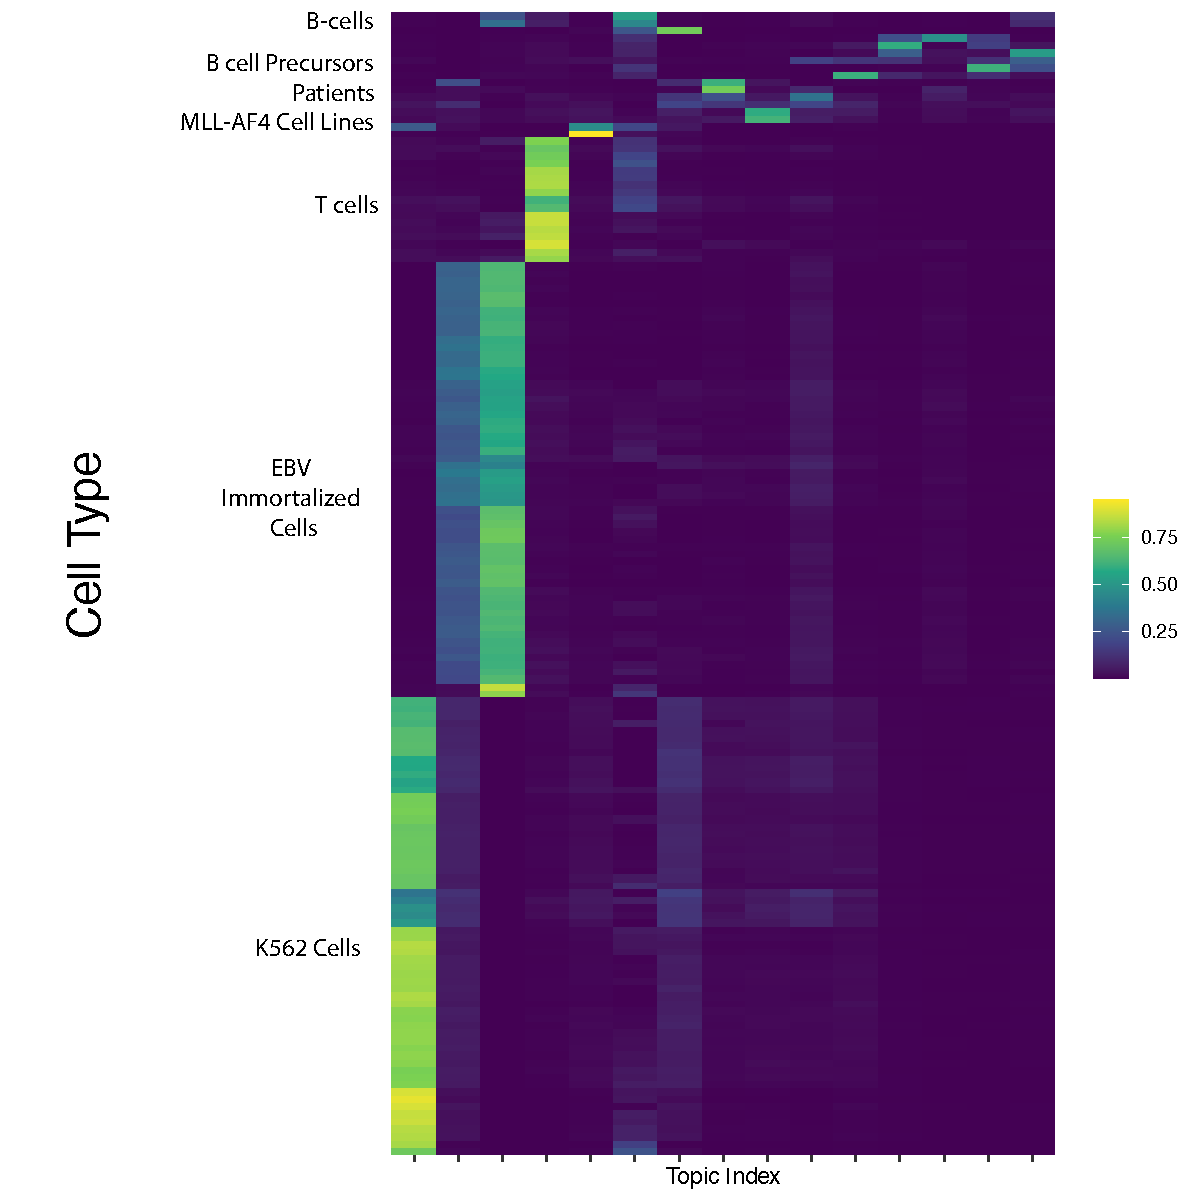
\includegraphics[width=\textwidth]{plot/ch5/mll_encode_nt15 _annotated.pdf}
%\end{figure}